\chapter{Binary Phase-Shift Keying (BPSK)}
\label{ch:bpsk}

\begin{nontechnical}
\textbf{BPSK is like Morse code with a twist}---instead of turning a signal on and off, you flip the wave upside-down to send 1s and 0s.

\textbf{Simple idea:}
\begin{itemize}
\item Bit 0 = wave pointing ``up'' $\uparrow$
\item Bit 1 = wave pointing ``down'' $\downarrow$ (flipped $180°$)
\end{itemize}

\textbf{Real use:} GPS satellites use BPSK! Your phone detects whether the signal is normal or flipped.

\textbf{Why flip instead of on/off?} More reliable in noise, works with constant power, less interference. Trade-off: Simple but slow (1 bit per symbol).
\end{nontechnical}

\section{Overview}

\textbf{Binary Phase-Shift Keying (BPSK)} is the simplest form of phase modulation, where binary data is encoded by shifting the carrier phase between two states: $0°$ and $180°$.

\textbf{Key advantage over OOK and FSK:} BPSK uses coherent detection and provides 3~dB better performance (lower BER for same SNR).

\textbf{Foundation for:} QPSK (4 phases), 8PSK (8 phases), and higher-order modulation schemes.

\section{Mathematical Description}

\subsection{Time-Domain Signal}

The BPSK waveform is expressed as:
\begin{equation}
s(t) = A \cos(2\pi f_c t + \phi_n)
\end{equation}
where:
\begin{itemize}
\item $A$ = carrier amplitude
\item $f_c$ = carrier frequency
\item $\phi_n \in \{0°, 180°\}$ = phase for bit $n$
\end{itemize}

\textbf{Phase encoding:}
\begin{equation}
\phi_n = \begin{cases}
0° & \text{if bit = 0} \\
180° & \text{if bit = 1}
\end{cases}
\end{equation}

\textbf{Alternative representation} (using cosine identity):
\begin{equation}
s(t) = A \cdot d_n \cdot \cos(2\pi f_c t)
\end{equation}
where:
\begin{itemize}
\item $d_n \in \{+1, -1\}$ = bipolar data symbol
\item Bit 0 $\rightarrow$ $d_n = +1$ $\rightarrow$ $0°$ phase
\item Bit 1 $\rightarrow$ $d_n = -1$ $\rightarrow$ $180°$ phase (inverted carrier)
\end{itemize}

\begin{calloutbox}{Key Insight}
BPSK is effectively \textbf{amplitude modulation with bipolar data}---the carrier polarity flips between positive and negative.
\end{calloutbox}

\section{IQ Representation}

The baseband complex representation of BPSK is:
\begin{equation}
s(t) = \mathrm{Re}\{A \cdot d_n \cdot e^{j2\pi f_c t}\}
\end{equation}

\textbf{IQ components:}
\begin{itemize}
\item \textbf{I (In-phase):} $I_n = A \cdot d_n$ (either $+A$ or $-A$)
\item \textbf{Q (Quadrature):} $Q_n = 0$ (BPSK uses only the I axis)
\end{itemize}

\subsection{Constellation Diagram}

The BPSK constellation consists of two points on the real axis:

\begin{center}
\begin{tikzpicture}[scale=1.5]
% Axes
\draw[->] (-3,0) -- (3,0) node[right] {$I$ (Real)};
\draw[->] (0,-2) -- (0,2) node[above] {$Q$ (Imaginary)};

% Constellation points
\fill[NavyBlue] (-2,0) circle (3pt) node[below=5pt] {Bit 1: $(-A, 0)$};
\fill[NavyBlue] (2,0) circle (3pt) node[below=5pt] {Bit 0: $(+A, 0)$};

% Distance annotation
\draw[<->,red,thick] (-2,0.5) -- (2,0.5) node[midway,above] {$d = 2A$};

% Phase annotations
\node[above=15pt] at (2,0) {$0°$ phase};
\node[above=15pt] at (-2,0) {$180°$ phase};
\end{tikzpicture}
\end{center}

\textbf{Euclidean distance between symbols:} $d = 2A$

This maximum separation provides optimal noise immunity for binary modulation.

\section{Modulation and Demodulation}

\subsection{Transmitter (Modulator)}

\textbf{Block diagram:}

\begin{center}
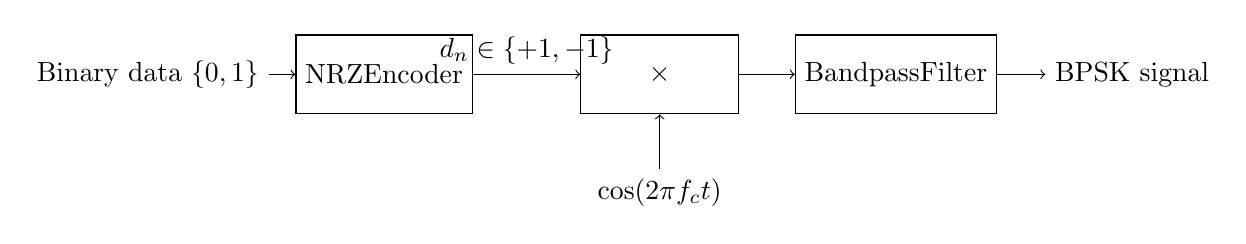
\begin{tikzpicture}[
  block/.style={rectangle, draw, minimum width=2cm, minimum height=1cm},
  node distance=2cm
]
\node (input) {Binary data $\{0, 1\}$};
\node[block, right of=input, node distance=3cm] (nrz) {NRZ\\Encoder};
\node[block, right of=nrz, node distance=3.5cm] (mult) {$\times$};
\node[block, right of=mult, node distance=3cm] (filter) {Bandpass\\Filter};
\node[right of=filter, node distance=3cm] (output) {BPSK signal};

\node[below of=mult, node distance=1.5cm] (carrier) {$\cos(2\pi f_c t)$};

\draw[->] (input) -- (nrz);
\draw[->] (nrz) -- node[above] {$d_n \in \{+1,-1\}$} (mult);
\draw[->] (carrier) -- (mult);
\draw[->] (mult) -- (filter);
\draw[->] (filter) -- (output);
\end{tikzpicture}
\end{center}

\textbf{Process:}
\begin{enumerate}
\item \textbf{NRZ encoding:} Map bits to symbols
  \begin{itemize}
  \item Bit 0 $\rightarrow$ $d_n = +1$
  \item Bit 1 $\rightarrow$ $d_n = -1$
  \end{itemize}
\item \textbf{Multiply by carrier:} $s(t) = A d_n \cos(2\pi f_c t)$
\item \textbf{Pulse shaping:} Apply raised-cosine filter to limit bandwidth and prevent intersymbol interference (ISI)
\end{enumerate}

\subsection{Receiver (Coherent Detector)}

\textbf{Block diagram:}

\begin{center}
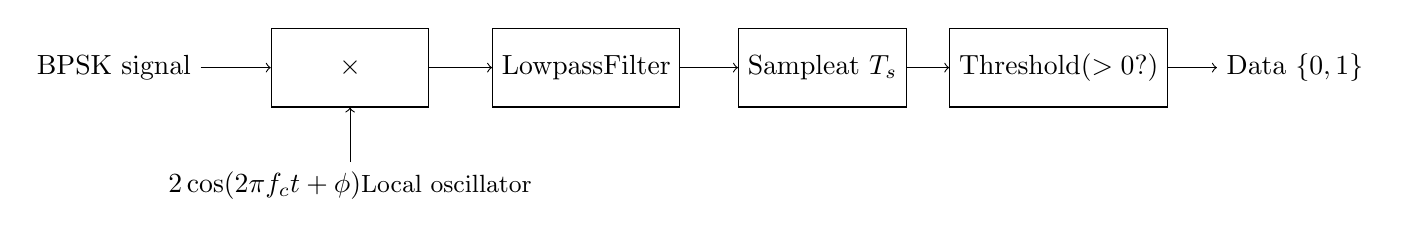
\begin{tikzpicture}[
  block/.style={rectangle, draw, minimum width=2cm, minimum height=1cm},
  node distance=2cm
]
\node (input) {BPSK signal};
\node[block, right of=input, node distance=3cm] (mult) {$\times$};
\node[block, right of=mult, node distance=3cm] (lpf) {Lowpass\\Filter};
\node[block, right of=lpf, node distance=3cm] (sample) {Sample\\at $T_s$};
\node[block, right of=sample, node distance=3cm] (thresh) {Threshold\\$(>0?)$};
\node[right of=thresh, node distance=3cm] (output) {Data $\{0,1\}$};

\node[below of=mult, node distance=1.5cm] (lo) {$2\cos(2\pi f_c t + \phi)$\\{\small Local oscillator}};

\draw[->] (input) -- (mult);
\draw[->] (lo) -- (mult);
\draw[->] (mult) -- (lpf);
\draw[->] (lpf) -- (sample);
\draw[->] (sample) -- (thresh);
\draw[->] (thresh) -- (output);
\end{tikzpicture}
\end{center}

\begin{calloutbox}[colback=red!5!white,colframe=red!75!black]{\textbf{WARNING:} Critical Requirement}
\textbf{Phase synchronization:} The local oscillator must be exactly in phase with the transmitter carrier. Phase offset causes signal degradation or complete loss.
\end{calloutbox}

\textbf{Detection process:}

\begin{enumerate}
\item \textbf{Multiply by local carrier} (same frequency and phase as TX):
\begin{equation}
r(t) = s(t) \cdot 2\cos(2\pi f_c t)
\end{equation}

\item \textbf{Product expansion:}
\begin{equation}
r(t) = A d_n \cos(2\pi f_c t) \cdot 2\cos(2\pi f_c t)
\end{equation}

\item \textbf{Apply trigonometric identity} $\cos(x)\cos(x) = \frac{1}{2}[1 + \cos(2x)]$:
\begin{equation}
r(t) = A d_n [1 + \cos(4\pi f_c t)]
\end{equation}

\item \textbf{Lowpass filter} removes $2f_c$ component:
\begin{equation}
r(t) = A d_n
\end{equation}

\item \textbf{Sample at bit period:} $y_n = A d_n + n(t)$ where $n(t)$ is noise

\item \textbf{Threshold decision:}
\begin{equation}
\hat{d}_n = \begin{cases}
+1 & \text{if } y_n > 0 \quad \text{(decode as bit 0)} \\
-1 & \text{if } y_n < 0 \quad \text{(decode as bit 1)}
\end{cases}
\end{equation}
\end{enumerate}

\section{Carrier Recovery}

\textbf{Problem:} The receiver must generate a local oscillator \textbf{exactly in phase} with the transmitter carrier.

A phase offset $\phi_e$ reduces the detected signal amplitude:
\begin{equation}
r(t) = A d_n \cos(\phi_e)
\end{equation}

If $\phi_e = 90°$: $r(t) = 0$ (complete signal loss!)

\subsection{Carrier Recovery Techniques}

\subsubsection{1. Pilot Tone}
\begin{itemize}
\item TX sends unmodulated carrier alongside data
\item RX phase-locks to pilot using a Phase-Locked Loop (PLL)
\item \textbf{Disadvantage:} Wastes power and bandwidth
\end{itemize}

\subsubsection{2. Costas Loop}
\begin{itemize}
\item PLL-based carrier recovery from the modulated signal itself
\item Multiplies received signal by both $\sin(2\pi f_c t)$ and $\cos(2\pi f_c t)$
\item Adjusts phase until Q-channel (sine branch) equals zero
\item \textbf{Advantage:} No pilot tone needed
\item \textbf{Disadvantage:} Complex implementation
\end{itemize}

\subsubsection{3. Squaring Loop}
\begin{itemize}
\item Square the BPSK signal: $(d_n \cos\theta)^2 = \frac{1}{2}d_n^2[1 + \cos(2\theta)]$
\item Since $d_n^2 = 1$, a doubled-frequency unmodulated carrier emerges
\item PLL locks to $2f_c$, then frequency is divided by 2
\item \textbf{Advantage:} Removes data modulation completely
\item \textbf{Disadvantage:} $180°$ phase ambiguity requires differential encoding
\end{itemize}

\subsection{Differential BPSK (DBPSK)}

\textbf{Solution to phase ambiguity:} Encode data in phase \textbf{transitions}, not absolute phase.

\textbf{Encoding:}
\begin{equation}
\phi_n = \phi_{n-1} + \Delta\phi_n
\end{equation}
where:
\begin{itemize}
\item Bit 0 $\rightarrow$ No phase change ($\Delta\phi = 0°$)
\item Bit 1 $\rightarrow$ Phase change ($\Delta\phi = 180°$)
\end{itemize}

\textbf{Decoding:} Compare consecutive symbols:
\begin{equation}
\hat{b}_n = \begin{cases}
0 & \text{if } \mathrm{sgn}(y_n) = \mathrm{sgn}(y_{n-1}) \\
1 & \text{if } \mathrm{sgn}(y_n) \neq \mathrm{sgn}(y_{n-1})
\end{cases}
\end{equation}

\begin{itemize}
\item \textbf{✓ Advantage:} No carrier recovery needed
\item \textbf{✗ Disadvantage:} Approximately 3~dB worse performance than coherent BPSK
\end{itemize}

\section{Bit Error Rate (BER) Performance}

\subsection{Coherent BPSK in AWGN Channel}

For ideal coherent detection in Additive White Gaussian Noise:
\begin{equation}
\mathrm{BER} = Q\left(\sqrt{\frac{2E_b}{N_0}}\right) = \frac{1}{2}\mathrm{erfc}\left(\sqrt{\frac{E_b}{N_0}}\right)
\end{equation}
where:
\begin{itemize}
\item $E_b$ = energy per bit = $\frac{A^2 T_b}{2}$
\item $N_0$ = noise power spectral density
\item $Q(x) = \frac{1}{\sqrt{2\pi}}\int_x^\infty e^{-t^2/2}\,dt$ (Gaussian tail probability)
\end{itemize}

\textbf{Key performance values:}

\begin{center}
\begin{tabular}{@{}lr@{}}
\toprule
$E_b/N_0$ (dB) & BER \\
\midrule
0~dB & $7.9 \times 10^{-2}$ (1 error in 13 bits) \\
5~dB & $9.7 \times 10^{-4}$ (1 in 1,000) \\
10~dB & $3.9 \times 10^{-6}$ (1 in 250,000) \\
15~dB & $6.9 \times 10^{-10}$ (1 in 1.4 billion) \\
\bottomrule
\end{tabular}
\end{center}

\subsection{Comparison: BPSK vs OOK}

At the same $E_b/N_0$:

\begin{center}
\begin{tabular}{@{}lr@{}}
\toprule
Modulation & BER @ 10~dB $E_b/N_0$ \\
\midrule
OOK (non-coherent) & $4.0 \times 10^{-3}$ \\
\textbf{BPSK (coherent)} & $\mathbf{3.9 \times 10^{-6}}$ \\
\bottomrule
\end{tabular}
\end{center}

\begin{calloutbox}[colback=green!5!white,colframe=green!75!black]{ Performance Advantage}
\textbf{BPSK is approximately 1000$\times$ better than OOK at 10~dB!}

\textbf{Why?}
\begin{enumerate}
\item BPSK uses both halves of signal space ($\pm A$ vs OOK's $\{0, A\}$)
\item Coherent detection (correlates with carrier---optimal receiver)
\item Maximum Euclidean distance between symbols
\end{enumerate}
\end{calloutbox}

\subsection{Differential BPSK Performance}

DBPSK has slightly worse performance than coherent BPSK:
\begin{equation}
\mathrm{BER}_{\mathrm{DBPSK}} \approx \frac{1}{2}e^{-E_b/N_0}
\end{equation}

At 10~dB $E_b/N_0$: BER $\approx 5 \times 10^{-6}$ (approximately 1.3~dB penalty vs coherent)

\section{Bandwidth Efficiency}

The occupied bandwidth (containing 99\% of power) is approximately:
\begin{equation}
B \approx \frac{1}{T_b} = R_b
\end{equation}
where $R_b$ is the bit rate in bits per second.

With raised-cosine pulse shaping (roll-off factor $\alpha$):
\begin{equation}
B = R_b(1 + \alpha)
\end{equation}

\textbf{Typical value:} $\alpha = 0.35$ gives $B = 1.35 R_b$

\textbf{Spectral efficiency:}
\begin{equation}
\eta = \frac{R_b}{B} = \frac{1}{1+\alpha} \approx 0.74\ \text{bps/Hz}
\end{equation}

\begin{calloutbox}{Example}
A 1~Mbps BPSK signal with $\alpha = 0.35$ requires \textbf{1.35~MHz} of bandwidth.
\end{calloutbox}

\section{Practical Implementations}

\subsection{IEEE 802.15.4 (Zigbee, Low-Rate WPAN)}

\textbf{PHY layer} (868/915~MHz bands):
\begin{itemize}
\item \textbf{Modulation:} BPSK (optional O-QPSK in 2.4~GHz band)
\item \textbf{Chip rate:} 300~kcps (868~MHz), 600~kcps (915~MHz)
\item \textbf{Data rate:} 20~kbps (868~MHz), 40~kbps (915~MHz)
\item \textbf{Spreading:} Direct-Sequence Spread Spectrum (DSSS)
\end{itemize}

\subsection{Satellite Telemetry}

Deep-space missions (Voyager, Mars rovers):
\begin{itemize}
\item \textbf{Modulation:} BPSK or QPSK
\item \textbf{Coding:} Convolutional + Reed-Solomon (concatenated FEC)
\item \textbf{Data rate:} 10~bps to 10~kbps (extreme distances)
\item \textbf{Why BPSK?} Maximum power efficiency---every dB counts at interplanetary distances
\end{itemize}

\begin{calloutbox}[colback=blue!5!white,colframe=blue!75!black]{ Voyager 1 Example}
At 24 billion km from Earth:
\begin{itemize}
\item TX power: 23~W
\item Antenna gain: 48~dBi (dish)
\item RX antenna: 70~m Deep Space Network dish (74~dBi)
\item Link budget: Barely positive with FEC (BER $\sim 10^{-5}$)
\end{itemize}
\end{calloutbox}

\subsection{RFID (Passive Tags)}

\textbf{Backscatter modulation:}
\begin{itemize}
\item Tag reflects or absorbs carrier energy
\item Binary encoding: reflection = bit 0, absorption = bit 1
\item Effectively BPSK from the reader's perspective
\item Data rate: 40--640~kbps (EPC Gen2 standard)
\end{itemize}

\section{Advantages of BPSK}

\begin{enumerate}
\item \textbf{Best BER performance} for binary modulation (3~dB better than OOK)
\item \textbf{Constant envelope} (nonlinear amplifiers acceptable, no AM-PM distortion)
\item \textbf{Simple constellation} (two points---easy to visualize and implement)
\item \textbf{Foundation for higher-order PSK} (QPSK, 8PSK extend the concept)
\end{enumerate}

\section{Disadvantages of BPSK}

\begin{enumerate}
\item \textbf{Requires carrier synchronization} (Costas loop or squaring loop adds complexity)
\item \textbf{Differential BPSK} avoids synchronization but suffers 3~dB penalty
\item \textbf{Low spectral efficiency} (1 bit/symbol = maximum 1~bps/Hz)
\item \textbf{Higher-order modulation} (QPSK, 16-QAM) more efficient for high SNR channels
\end{enumerate}

\section{Transition to QPSK}

BPSK uses only the I-axis with two constellation points.

\textbf{Natural extension:} Use \textbf{both I and Q axes} to create QPSK:

\begin{center}
\begin{tikzpicture}[scale=1.2]
% BPSK
\begin{scope}[shift={(0,0)}]
\node[above] at (0,2.5) {\textbf{BPSK}};
\draw[->] (-2,0) -- (2,0) node[right] {$I$};
\draw[->] (0,-1.5) -- (0,1.5) node[above] {$Q$};
\fill[NavyBlue] (-1.5,0) circle (2pt);
\fill[NavyBlue] (1.5,0) circle (2pt);
\node[below] at (0,-1.5) {2 points, 1 bit/symbol};
\end{scope}

% QPSK
\begin{scope}[shift={(6,0)}]
\node[above] at (0,2.5) {\textbf{QPSK}};
\draw[->] (-2,0) -- (2,0) node[right] {$I$};
\draw[->] (0,-1.5) -- (0,1.5) node[above] {$Q$};
\fill[NavyBlue] (1.06,1.06) circle (2pt);
\fill[NavyBlue] (-1.06,1.06) circle (2pt);
\fill[NavyBlue] (-1.06,-1.06) circle (2pt);
\fill[NavyBlue] (1.06,-1.06) circle (2pt);
\node[below] at (0,-1.5) {4 points, 2 bits/symbol};
\end{scope}
\end{tikzpicture}
\end{center}

\textbf{QPSK} = Two independent BPSK channels (I and Q) operating in parallel, doubling spectral efficiency.

\section{Worked Example: BPSK Link Budget}

\textbf{Scenario:} Satellite downlink from geostationary orbit

\textbf{Given parameters:}
\begin{itemize}
\item TX power: $P_t = 10$~W (40~dBm)
\item TX antenna gain: $G_t = 30$~dBi
\item Distance: $d = 36{,}000$~km (GEO)
\item Frequency: $f = 12$~GHz (Ku-band)
\item RX antenna gain: $G_r = 40$~dBi (1~m dish)
\item System noise temperature: $T_s = 150$~K
\item Bandwidth: $B = 1$~MHz
\item Required BER: $10^{-6}$
\end{itemize}

\subsection{Step 1: Calculate Free-Space Path Loss}

\begin{equation}
\mathrm{FSPL} = 20\log_{10}(d) + 20\log_{10}(f) + 92.45
\end{equation}
\begin{equation}
\mathrm{FSPL} = 20\log_{10}(36 \times 10^6) + 20\log_{10}(12 \times 10^9) + 92.45 = 205.5\ \text{dB}
\end{equation}

\subsection{Step 2: Calculate Received Power}

\begin{equation}
P_r = P_t + G_t + G_r - \mathrm{FSPL}
\end{equation}
\begin{equation}
P_r = 40 + 30 + 40 - 205.5 = -95.5\ \text{dBm}
\end{equation}

\subsection{Step 3: Calculate Noise Power}

\begin{equation}
N = kT_sB = (1.38 \times 10^{-23})(150)(10^6) = 2.07 \times 10^{-15}\ \text{W} = -117\ \text{dBm}
\end{equation}

\subsection{Step 4: Calculate SNR}

\begin{equation}
\mathrm{SNR} = P_r - N = -95.5 - (-117) = 21.5\ \text{dB}
\end{equation}

\subsection{Step 5: Verify BER Requirement}

For BPSK at BER $= 10^{-6}$, we require $E_b/N_0 \approx 10.5$~dB.

Convert SNR to $E_b/N_0$:
\begin{equation}
\frac{E_b}{N_0} = \mathrm{SNR} + 10\log_{10}\left(\frac{B}{R_b}\right)
\end{equation}

If data rate $R_b = 500$~kbps:
\begin{equation}
\frac{E_b}{N_0} = 21.5 + 10\log_{10}\left(\frac{10^6}{5 \times 10^5}\right) = 21.5 + 3 = 24.5\ \text{dB}
\end{equation}

\begin{calloutbox}[colback=green!5!white,colframe=green!75!black]{✓ Link Margin}
\textbf{Available $E_b/N_0$:} 24.5~dB

\textbf{Required $E_b/N_0$:} 10.5~dB

\textbf{Margin:} $24.5 - 10.5 = 14$~dB

This comfortable margin accommodates rain fade, implementation loss, and other impairments. \textbf{Link closes successfully!}
\end{calloutbox}

\section{Summary}

\begin{center}
\begin{tabular}{@{}ll@{}}
\toprule
\textbf{Aspect} & \textbf{BPSK} \\
\midrule
Bits per symbol & 1 \\
Constellation points & 2 ($0°$, $180°$) \\
Spectral efficiency & $\sim$1~bps/Hz (with pulse shaping) \\
BER @ 10~dB $E_b/N_0$ & $3.9 \times 10^{-6}$ \\
Carrier recovery & Required (Costas loop, squaring loop) \\
Complexity & Moderate (coherent detection) \\
Best application & Power-limited channels (satellite, deep-space) \\
\bottomrule
\end{tabular}
\end{center}

\section{Further Reading}

\begin{itemize}
\item \textbf{Chapter \ref{ch:ook}:} On-Off Keying---simpler but 3~dB worse performance
\item \textbf{Chapter \ref{ch:fsk}:} Frequency-Shift Keying---alternative binary modulation
\item \textbf{Chapter \ref{ch:qpsk}:} QPSK---extension to 4 phases (2 bits/symbol)
\item \textbf{Chapter \ref{ch:constellation-diagrams}:} Constellation Diagrams---visual representation
\item \textbf{Chapter \ref{ch:iq-representation}:} IQ Representation---complex baseband notation
\item \textbf{Chapter \ref{ch:ber}:} Bit Error Rate analysis and measurement
\item \textbf{Chapter \ref{ch:fec}:} Forward Error Correction for improved BER
\end{itemize}
